% !TeX root = RJwrapper.tex
\title{The MD in .Rmd: Teaching Clinicians Data Analytics with R}
\author{by Ted Laderas and Brian Sikora}

\maketitle

\abstract{%
Data Analytics in Healthcare is difficult to teach effectively,
especially to clinical professionals. In this article, we outline our
Data Analytics course and our strategies for effective learning of both
practical data science skills (SQL and modeling in R) and strategies for
effectively presenting analyses within an healthcare organization using
a readmission metric. We highlight the creative ways our students
present their results and the impact the course has made on them.
}

\hypertarget{introduction}{%
\subsection{Introduction}\label{introduction}}

Delivering analytics effectively in healthcare is a difficult concept to
teach effectively. Key practical data science skills (such as querying,
visualizing, and modeling real data) must be combined with
organizational thinking. In this article, we outline our Data Analytics
course which focuses two aspects of analytics: organizational
considerations and practical R skills.

This course is unique in that it has both clinical informatics and
bioinformatics students within our departments. We take advantage of
this mixed audience to build a support structure for both the clinicians
and the bioinformatics students.

By the end of the course, our students must synthesize both of these
branches by querying and modeling the data and present their results to
an Executive team.

\hypertarget{clinicians-as-learners}{%
\subsection{Clinicians as Learners}\label{clinicians-as-learners}}

In our past 6 years teaching the course, we have honed our understanding
of clinicians as learners. We have built our learner persona as Mary:

\begin{quote}
Mary is a clinician who wants to understand how analytics can be
delivered in her healthcare organization. She \emph{has little time},
and likes \emph{learning on her own}. She has a \emph{hard time asking
for help} and can be overly self critical.
\end{quote}

We have tailored the material in the course to accommodate the learners
{[}in the following ways{]}:

\emph{Mary has little time} - our assignments utilize a lot of ``just in
time'' instruction. For instance, each assignment focuses on a key
concept that builds on previous concepts, such as single table queries
first, followed by table joins, and self-joins. Additionally, the
assignments slowly increase in difficulty.

\emph{Mary likes learning on her own} - all assignments are delivered as
RMarkdown documents within Rstudio projects and distributed via
RStudio.cloud. The ease of setup with RStudio.cloud gets our students up
and running relatively quickly. Delivering individual assignments as
projects allows us to pace the tempo of learning, and focus them on
particular topics.

\emph{Mary has a hard time asking for help}. We attempt to destigmatize
asking for help with the following strategies: team-based learning,
office hours, and individual appointments.

\hypertarget{simulating-data-analytics}{%
\subsection{Simulating Data Analytics}\label{simulating-data-analytics}}

Our course centers around a single analytical task: predicting
readmissions in a simulated patient population using a validated metric,
LACE. {[}{]} LACE is short for

\begin{itemize}
\tightlist
\item
  \textbf{L}ength of Stay
\item
  \textbf{Acuity} of Admission
\item
  \textbf{Comorbidities}
\item
  \textbf{Emergency Room} Visits
\end{itemize}

In order to calculate these, a number of assignments center around
exploring, extracting, querying, summarizing, modeling, and presenting
the patient information (Figure \ref{fig:assignments}).

The expectation is that students not only utilize their practical
skills, but make it understandable to an executive team. Our assignments
center around querying and calculating the LACE metric for a simulated
clinical warehouse. This clinical warehouse is stored as a SQLite
Database and is accessed through the R Projects using the \texttt{DBI}
and \texttt{RSQLite} packages. It represents a clinical extract of
patients admitted into the hospital, along with their diagnoses.

\begin{Schunk}
\begin{figure}

{\centering \subfloat[Exploratory Data Analysis\label{fig:assignments-1}]{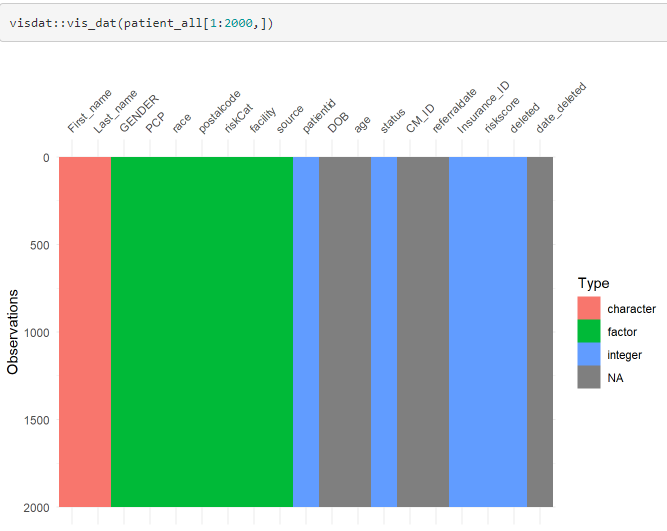
\includegraphics[width=0.5\linewidth]{C:/Code/rmed_2020_talk/image/visdat} }\subfloat[SQL Queries\label{fig:assignments-2}]{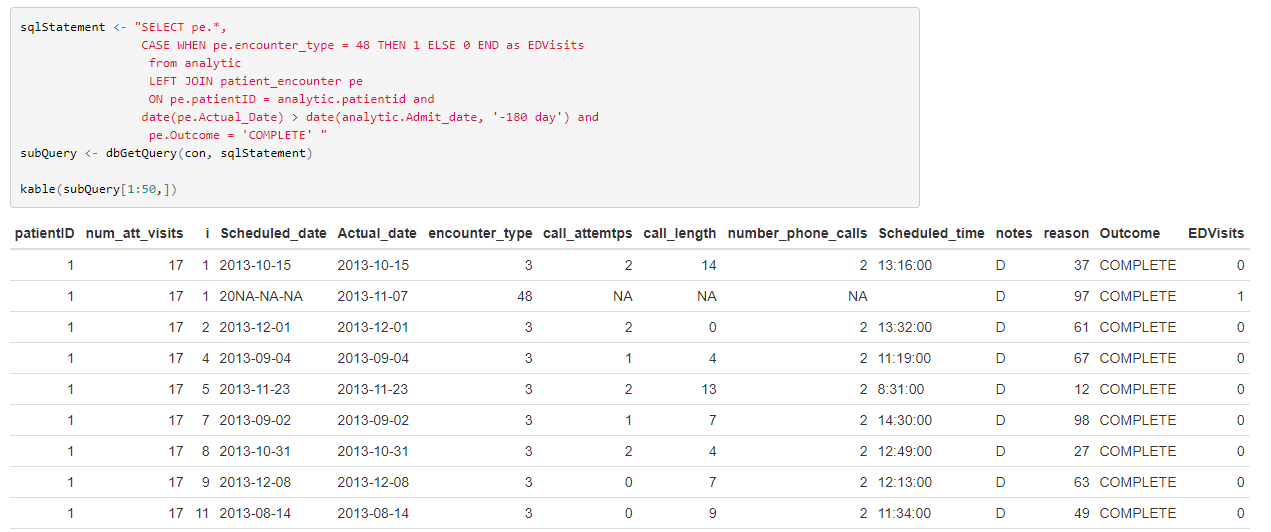
\includegraphics[width=0.5\linewidth]{C:/Code/rmed_2020_talk/image/sql2} }\newline\subfloat[Logistic Regression\label{fig:assignments-3}]{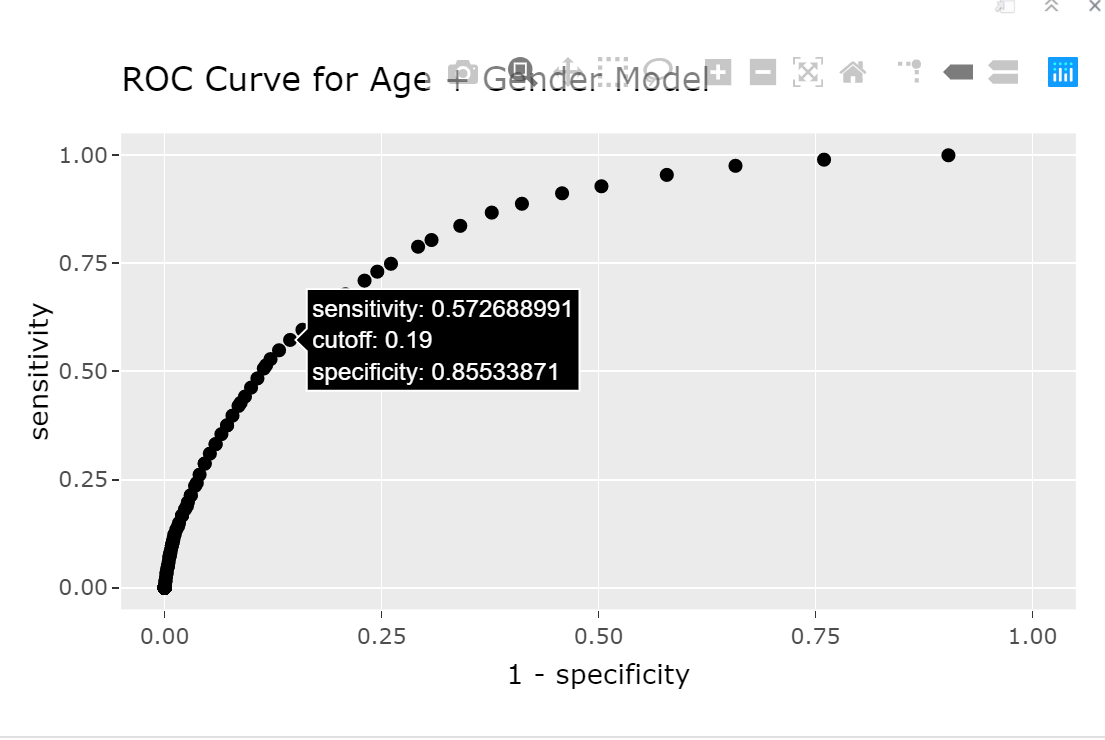
\includegraphics[width=0.5\linewidth]{C:/Code/rmed_2020_talk/image/roc-curve} }\subfloat[Machine Learning\label{fig:assignments-4}]{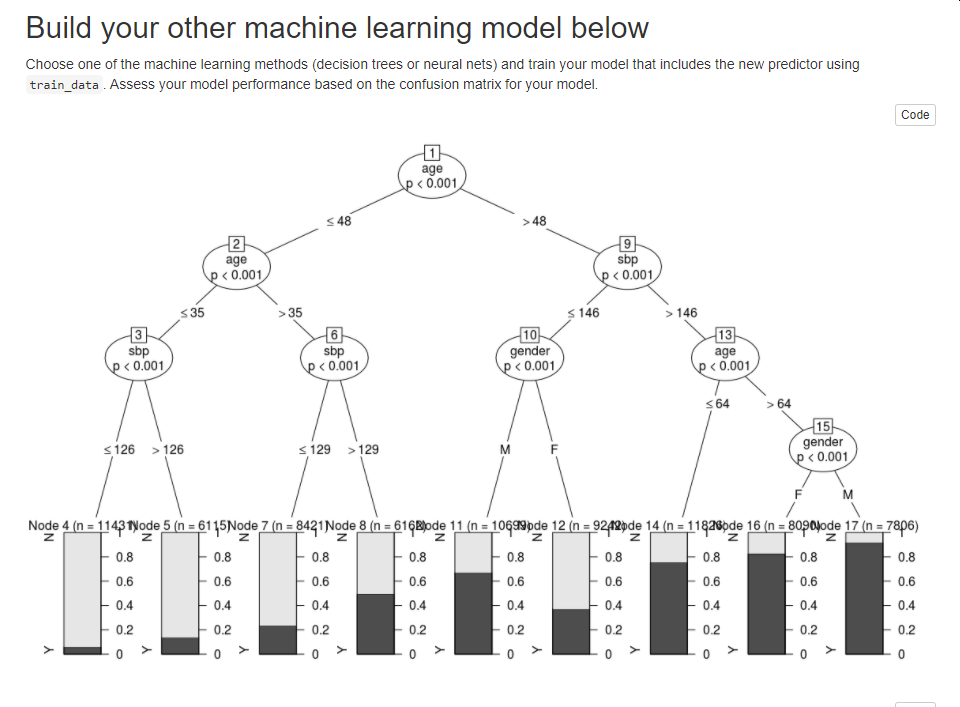
\includegraphics[width=0.5\linewidth]{C:/Code/rmed_2020_talk/image/ml} }

}

\caption[Analytics Assignments, in order of difficulty]{Analytics Assignments, in order of difficulty}\label{fig:assignments}
\end{figure}
\end{Schunk}

The assignments progress in order of difficulty:

Exploratory Data Analysis: Use tools such as \texttt{visdat} and
\texttt{skimr} to explore the structure of the tables in the data
warehouse and missing values. (Figure \ref{fig:assignments}a)

SQL Queries: start with simple one table queries, graduate to multi join
queries, including self-joins and counts (Figure \ref{fig:assignments}b)

Calculating individual components: calculate and document how to
calculate each component of the LACE Score. These assignments require
multi table queries, including querying the \texttt{patient},
\texttt{patient\_encounter\_hosp}, and \texttt{patient\_diagnosis}
tables within the database to aggregate and summarize these LACE
components for each patient.

Modeling: build a logistic regression model or a machine learning model
to predict readmission in the simulated patient population (Figure
\ref{fig:assignments}c).

Visualization: use \texttt{ggplot2} and other \texttt{tidyverse}
packages to visualize outcomes and association with covariates.

\hypertarget{organizational-skills-and-challenges}{%
\subsection{Organizational Skills and
Challenges}\label{organizational-skills-and-challenges}}

Equally important skills for Analysts are effectively aligning analytic
projects to the strategic goals within an organization (Figure
\ref{fig:organization}). To this end, we provide lectures in
organizational behavior topics such as finding organizational sponsors,
establishing analytic priorities, understanding organizational dynamics
and culture, change management in an organization, evaluating the
clinical utility of a metric, as well as the lifecycle of analytic
projects in an organization. These lectures are supplemented by reading
assignments {[}{]} and online and in-class discussion of these topics.

The organizational skills lectures are delivered by guest lecturers from
Kaiser Permanente, who share their own experiences of working as an
effective analytic team within Kaiser Permanente. Most importantly, the
experience of implementing LACE as a useful metric within KP is
highlighted.

In particular, the first implementation of LACE at KP was a failure, and
students get the opportunity to learn about why the first implementation
was not successful. The second successful implementation of LACE
highlights essential change management skills needed to make LACE a
success within KP as an organization.

Students have found these lectures to be helpful in understanding the
context of delivering their analyses.

\begin{Schunk}
\begin{figure}

{\centering 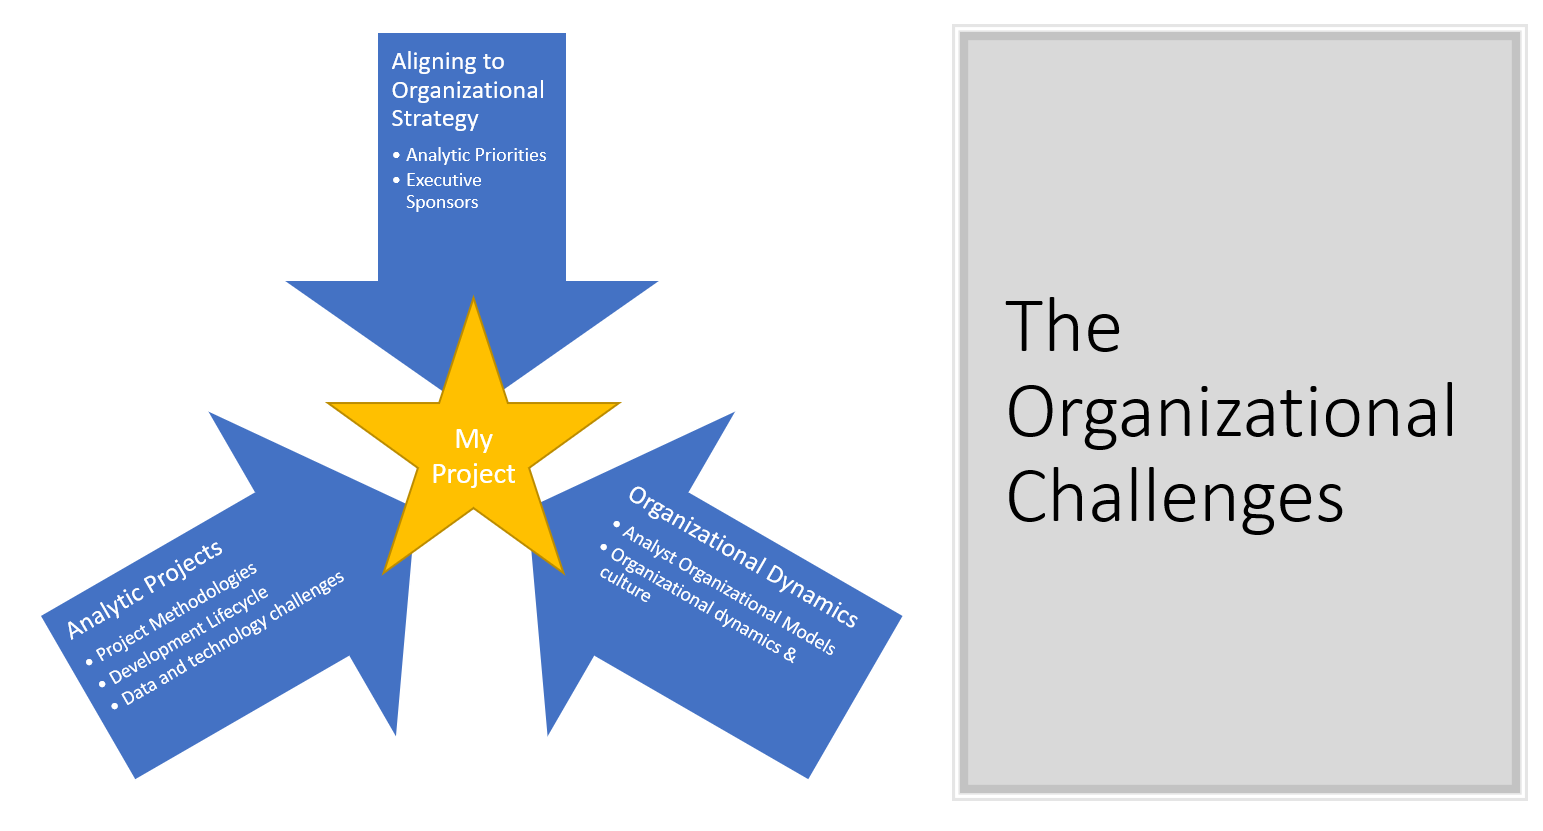
\includegraphics[width=0.5\linewidth]{C:/Code/rmed_2020_talk/image/org_challenges} 

}

\caption[Organizational Challenges in delivering Data Analytics]{Organizational Challenges in delivering Data Analytics}\label{fig:organization}
\end{figure}
\end{Schunk}

\hypertarget{final-presentation}{%
\subsection{Final Presentation}\label{final-presentation}}

The final presentations consists presenting their modeling results and
findings to a healthcare organization. The instructors role play as
executive sponsors within a fictional healthcare organization. The
students are expected to interpret and present a model meaningfully in a
way that aligns with organizational goals. The presentation needs to be
pitched in a way that is accessible to executives.

In order to facilitate this, we have developed lectures both in
organizational considerations in presenting data, data storytelling with
visuals, and provided a template for effectively presenting the data.

\hypertarget{outcomes-creativity-in-presentations}{%
\subsection{Outcomes: Creativity in
Presentations}\label{outcomes-creativity-in-presentations}}

\begin{Schunk}
\begin{figure}

{\centering \subfloat[Enhanced version of LACE\label{fig:presentations-1}]{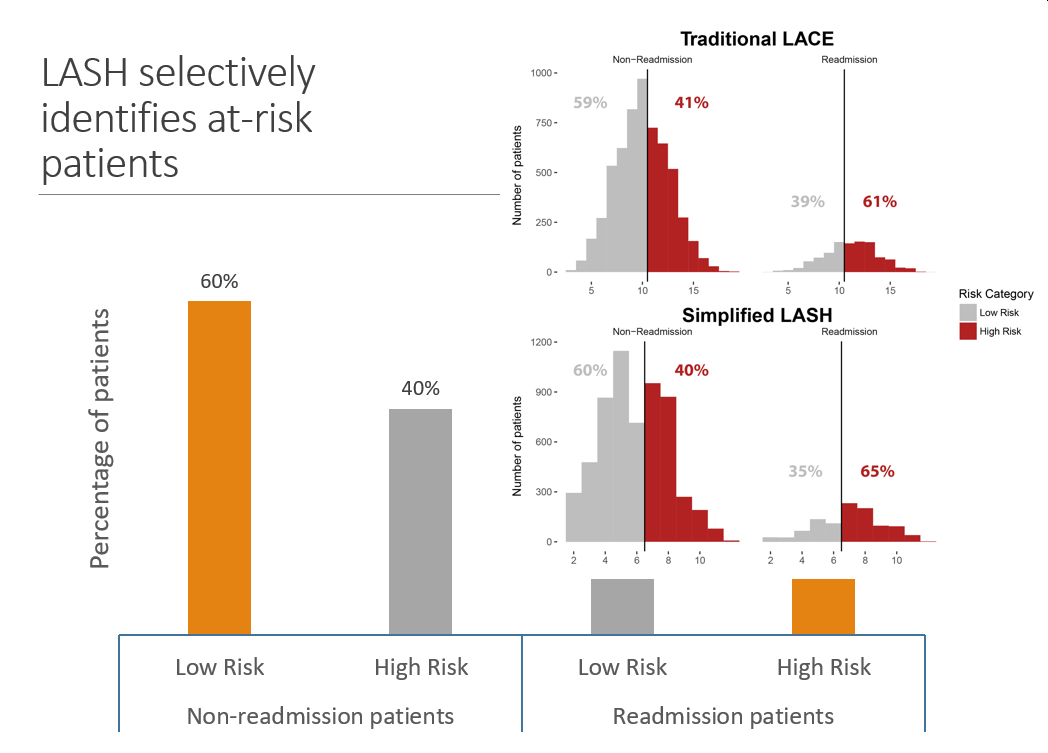
\includegraphics[width=0.5\linewidth]{C:/Code/rmed_2020_talk/image/watanabe-meenakashi} }\subfloat[Selecting a threshold using a Cost Metric\label{fig:presentations-2}]{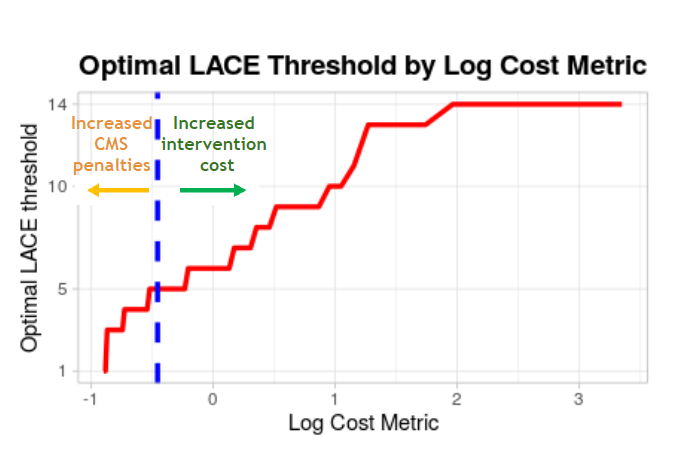
\includegraphics[width=0.5\linewidth]{C:/Code/rmed_2020_talk/image/nguyen-yaeger-wang} }\newline\subfloat[Summarizing the cost/savings of using LACE\label{fig:presentations-3}]{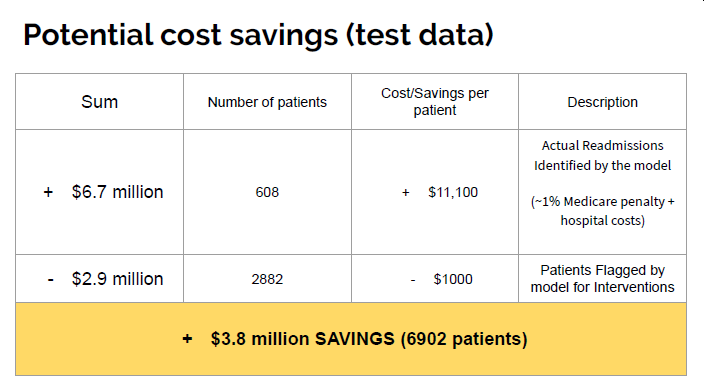
\includegraphics[width=0.5\linewidth]{C:/Code/rmed_2020_talk/image/grout-lin-xu} }

}

\caption[Final presentations of LACE]{Final presentations of LACE}\label{fig:presentations}
\end{figure}
\end{Schunk}

Based on our template, student teams have come up with creative ways of
presenting their models to the executive team (Figure
\ref{fig:presentations}).

\hypertarget{outcomes-testimonies}{%
\subsection{Outcomes: Testimonies}\label{outcomes-testimonies}}

Students have been highly receptive to the course. In a recent
curriculum committee meeting, both the Clinical and Bioinformatics
student representatives recommended that this course be taught to all
students in the department.

Interviews with students about the course have featured the following
themes:

\emph{Collaboration}:

\begin{quote}
Taking the Data Analytics course made me a \textbf{much more patient and
effective collaborator}, especially when working with colleagues outside
of science.
\end{quote}

--- Kristen Stevens, MD/PhD Candidate

\emph{Diversity}:

\begin{quote}
I highly recommend this course to anyone who wishes to get a
comprehensive introduction to R and the field of data analytics.
.b{[}The course attracts {[}a{]} very diverse set of students.{]} The
hybrid nature of the course was ideal to get to meet and network with
others.
\end{quote}

--- Meenakashi Mishra, Clinical Informatics Fellow

\emph{Comprehensive view of the field}:

\begin{quote}
I would definitely recommend this to .b{[}anyone who is interested in
working with data in a healthcare setting{]}, whether you're a
clinician/researcher who will be gathering and using the data, or a
manager who might be presenting the data or incorporating analytics into
your organization's workflow.
\end{quote}

--- Pierrette Lo, Biomedical Project Manager/Data Scientist

\emph{The Future}:

\begin{quote}
As a clinician, to see how a data analysis works and how algorithms
result in a recommendation was very helpful. \ldots. informatics
programs \textbf{should expand their technical analytics courses for
clinicians and other clinical informatics students}. Perhaps some day
there will be a formal role for clinician-data scientists in the
healthcare industry outside of research, and if there will be it starts
with courses like this.
\end{quote}

--- Frank Longano, MD, Clinician

\hypertarget{conclusions}{%
\subsection{Conclusions}\label{conclusions}}

Over six years of giving this course to both clinicians and
bioinformaticians, we have honed the art of conducting analysis and
making it accessible and actionable within a healthcare organization.
Our two-pronged approach of teaching both practical data science skills
and organizational skills

\hypertarget{availability}{%
\subsection{Availability}\label{availability}}

All code for the individual RStudio Projects are available here:
\url{https://github.com/laderast/AnalyticsCourse}

\bibliography{md-rmd-paper.bib}

\address{%
Ted Laderas\\
Medical Informatics and Clinical Epidemiology, Oregon Health \& Science
University\\%
3181 S.W. Sam Jackson Park Road, BICC\\ Portland, OR 97239, United
States of America\\
%
\url{https://laderast.github.io}%
\\\textit{ORCiD: \href{https://orcid.org/0000-0002-9079-593X}{0000-0002-9079-593X}}%
\\\href{mailto:tedladeras@gmail.com}{\nolinkurl{tedladeras@gmail.com}}
}

\address{%
Brian Sikora\\
Kaiser Permanente Insight\\%
line 1 affiliation 1\\ line 2 affiliation 1\\
%
\url{https://journal.r-project.org}%
\\\textit{ORCiD: \href{https://orcid.org/0000-0002-9079-593X}{0000-0002-9079-593X}}%
\\\href{mailto:author2@work}{\nolinkurl{author2@work}}
}
